\subsection{Schnyder-Wood-Fluss}

Um einen Schnyder Wood als Fluss-Problem zu kodieren, kann man die in Abschnitt \ref{alpha_orientations} eingeführten $\alpha_s$-Orientierungen auf dem Abschluss von $G+G^*$ nutzen. Fusy zeigt in \cite{fusy07} im Zuge der Untersuchung spezifischer $\alpha$-Funktionen, dass sich $\alpha_s$-Orientierungen von $G+G^*$ in linearer Zeit berechnen lassen, sodass wir auch einen Schnyder Wood auf $G$ in linearer Zeit erhalten.\\

Machen wir uns also an die Konstruktion eines Netzwerks $\mathcal{N}_S$, sodass ein zulässiger ganzzahliger Fluss $\varphi_s$ einer $\alpha_s$-Orientierung von $G+G^*$ entspricht. Nach Theorem \ref{alpha_bij} induziert $\varphi_s$ somit auch einen Schnyder Wood auf $G$. Besonderes Augenmerk ist hier auf die Möglichkeit einer späteren Kombination mit einem FAA-Fluss gelegt, um ein Kombiniertes Netzwerk zu erstellen, und nicht unbedingt auf Effizienz.

Wie oben schon erwähnt ist $G+G^*$ bipartit, Kanten-Knoten haben Grad 4, Knoten-Knoten Grad $deg(v)$ und Gebiets-Knoten Grad $|f|$. Für eine $\alpha_s$-Orientierung muss nach Definition \ref{alpha_bij} A3 jeder Kanten-Knoten Ausgrad 1, jeder Knoten-Knoten Eingrad $deg(v)-3$ und jeder Gebiets-Knoten Eingrad $|f|-3$ haben. Die Kanten-Knoten am äusseren Gebiet sind in $G+G^*$ immer nach aussen orientiert. Somit können wir nur die inneren Kanten-Kanten $E_{in}$ betrachten und die Orientiertung der äusseren Kanten voraus setzten.

\begin{figure}[h]
	\centering
  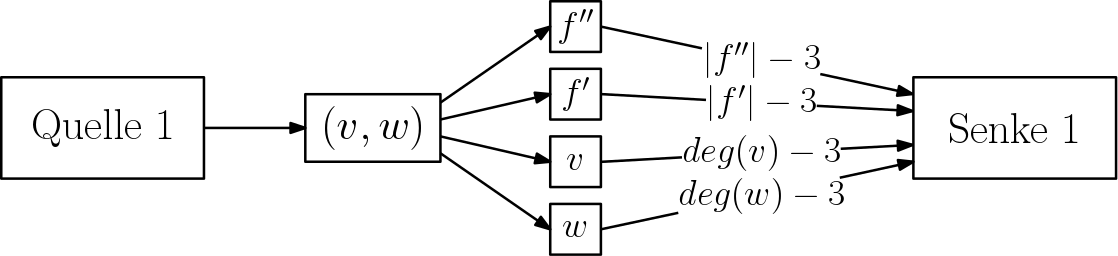
\includegraphics[width=0.9\textwidth]{schnyder_flow.png}
  \caption{Der Schnyder Wood Fluss durch eine innere Kante $(v,w)$.}
  \label{schnyder_flow}
\end{figure}

Sei $\mathcal{N}_S$ ein Netzwerk mit jeweils einer Quelle $s$ und Senke $t$, Kanten von der Quelle zu jedem $e \in E_{in}$ mit Kapazität 1, Kanten von den Kanten-Knoten $e$ zu inzidenten Knoten-Knoten $v$ und (inneren) Gebiets-Knoten $f \in F_{in}$ in $G$ ebenfalls mit Kapazität 1, Kanten von $f \in F_{in}$ zur Senke mit Kapazitäten $|f|-3$, Kanten von den (inneren) Knoten-Knoten $v \in V_{in} = V \setminus \{a_1,a_2,a_3\}$ zur Senke mit Kapazitäten $deg(v)-3$ und Kanten von den Aufhängungen $a_i$ zur Senke mit Kapazitäten $deg(a_i)-2$. Die letzte Kapazität resultiert aus dem Fakt, dass die Halbkante in $G+G^*$ von $a_i$ aus immer nach aussen orientiert ist und wir somit nur noch zwei andere Kanten nach aussen orientieren müssen.

Der Bedarf des Netzwerkes entspricht der Anzahl der inneren Kanten von $G$. Sei nun $\varphi_s$ eine zulässige ganzzahlige Lösung, dann hat jeder Kanten-Knoten $e$ Ausgrad 1. Der Fluss $\varphi_s$ entlang einer Auskante von $e \in E_{in}$ in $\mathcal{N}_S$ entspricht dann genau der hin zu $e$ orientierten Kante einer $\alpha_{s}$-Orientierung auf $G+G^*$. Die Knoten-Knoten und Gebiets-Knoten haben $deg(v)-3$ bzw. $|f|-3$ von $\varphi_S$ genutzte Auskanten und somit entspricht hier eine leere Kante in $\mathcal{N}_S$ einer von $v$ bzw. $f$ weg orientierten Kante bezüglich $\alpha_{s}$. Für einen zulässigen ganzzahligen Fluss $\varphi_s$ gilt $|\varphi_s| = |E_{in}|$. Somit hat jede innere Kante Ausgrad 1. Weiter gilt 
$$\sum_{v \in V} \Big(\text{deg}(v)-3\Big) + 3 + \sum_{f \in F_{in}} \Big(|f|-3\Big) = |E_{in}|.$$

Somit hat jedes Gebiet und jeder Knoten den passenden Ausgrad und $\varphi_s$ kodiert eine $\alpha_s$-Orientierung auf $G+G^*$. Es existiert also genau dann ein Schnyder Wood auf $G$, wenn eine ganzzahlige Lösung $\varphi_S$ für $\mathcal{N}_S$ existiert.

Fassen wir zusammen.

\begin{network}[Schnyder Wood]
Bei $\mathcal{N}_s$ handelt es sich um ein gerichtetes Netzwerk, das auf Basis von $G$ erstellt wird, um einen Schnyder Wood auf $G$ zu finden. Ein Ausschnitt ist in Abbildung \ref{schnyder_flow} dargestellt.
	\begin{itemize}
	\item $\mathcal{N}_s$ hat eine Quelle $s$ und eine Senke $t$
	\item Knoten in $\mathcal{N}_s$ werden für jeden innere Kante $e \in E_{in}$, jedes innere Gebiet $f\in F_{in}$ und jeden Knoten $v \in V$ aus $G$ erzeugt.
	\item Es werden gerichtete Kanten der folgenden Typen in $\mathcal{N}_S$ erzeugt:
		\begin{itemize}
		\item $(s,e)$ von der Quelle zu jeder inneren Kante mit $c\big(s,e\big) = 1$
		\item $(e,v_1),(e,v_2)$ von jeder inneren Kante zu den Endknoten mit $c\big(e,v\big) = 1$
		\item $(e,f)$ von jeder inneren Kante zu adjazenten Gebieten mit $c\big(e,f\big) = 1$
		\item $(f,t)$ von den inneren Gebieten zur Senke mit $c\big(f,t\big) = 1$
		\item $(v,t)$ von den Knoten zur Senke mit $c\big(v,t\big) = 1$
		\item $(f,t)$ von den inneren Gebieten zur Senke mit $c\big(f,t\big) = |f|-3$
		\item $(a_i,t)$ von den Aufhängungen zur Senke mit $c\big(f,t\big) = \text{deg}(a_i)-2$
		\item $(v,t)$ von den restlichen Knoten zur Senke mit $c\big(f,t\big) = \text{deg}(v)-3$
		\end{itemize}
	\item $\mathcal{N}_S$ hat Bedarf $d=|E_{in}|$
	\item [$\Rightarrow$] Ein zulässiger ganzzahliger Fluss $\varphi_s$ existiert. $\Leftrightarrow$ Es existiert ein Schnyder Wood  auf $G$.
	\end{itemize}
\end{network}	

\subsection{FAA-Fluss}\label{faa-flow}

Um ein FAA für einen planaren Graphen $G$ zu erhalten, müssen wir jedem Gebiet $f \in F$ genau drei Ecken und $|f|-3$ flache Winkel zuordnen. Jeder Knoten darf maximal einem Gebiet zugeordnet werden, also in diesem flach sein. Falls eine Einbettung und die Aufhängungen $\{a_1,a_2,a_3\}$ gegeben sind, müssen wir jedem inneren Gebiet $f \in F_{in}$ drei Ecken und $|f|-3$ flache Winkel zuweisen und jeder innere Knoten $v \in V_{in}$ darf maximal einem Gebiet zugeordnet werden. Die Knoten um das äussere Gebiet die keine Aufhängungen sind müssen diesem zugewiesen werden. Wir konstruieren ein Netzwerk für den zweiten Fall, das sich leicht verallgemeinern lässt.\

Sei also wieder $\mathcal{N}_F$ ein Netzwerk mit einer Quelle und Senke. Wir erstellen in $\mathcal{N}_F$ Knoten für jeden inneren Winkel $(f,v)$, mit $v\in V$ und $f \in F_{in}$, Knoten für alle inneren Gebiete $f \in F_{in}$ und alle Knoten $v\in V$. Von der Quelle existiert eine Kante mit Kapazität 1 zu jedem inneren Winkel $(f,v)$, von jedem inneren Winkel $(f,v)$ jeweils eine Kante zu $f$ und zu $v$ mit Kapazität 1. Zuletzt fügen wir Kanten von jedem inneren Gebiet $f$ zur Senke mit Kapazität 3 und Kanten von jedem Knoten $v$ zur Senke mit Kapazität 1 ein. Der Bedarf des Netzwerks ist $\sum_{f \in F_{in}}{|f|}$ und entspricht der Anzahl der inneren Winkel von $G$.

\begin{figure}[h]
	\centering
  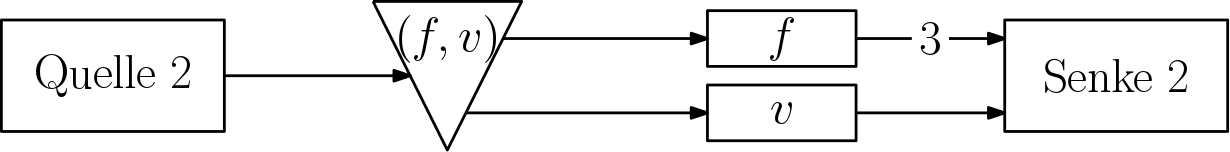
\includegraphics[width=0.8\textwidth]{faa_flow.png}
  \caption{Der FAA-Fluss durch einen Winkel $(f,v)$.}
  \label{faa_flow}
\end{figure}

Sei $\varphi_F$ ein zulässiger ganzzahliger Fluss, dann entspricht Fluss auf einer Kante $((f,v),f)$ einer Ecke (eines möglichen GFAAs) von $f$ und Fluss auf $((f,v),u)$ der Zuweisung eines Knoten zu $f$, also einem flachen Winkel in einem GFAA. Zur Vereinfachung sprechen wir im Weitern auch von Ecken- und Zuweisungs-Fluss. Somit wird jeder innere Winkel entweder seinem Gebiet zugewiesen oder als Ecke ausgezeichnet. An jedem inneren Knoten kann nur jeweils ein Winkel zugewiesen werden (F2). Von jedem inneren Gebiet $f$ fließt Fluss mir Stärke $|\varphi_s((f,t))| = |f|-3$ zu Senke. F1 ist als erfüllt. $\varphi_F$ respektiert also die Bedingungen aus Definition \ref{def_faa} und es existieren nur dann FAAs auf $G$, wenn mindestens eine ganzzahlige Lösung für $\mathcal{N}_F$ existiert. Eine spezifische Lösung $\varphi_F$ entspricht genau einem FAA auf $G$.

Fassen wir zusammen.

\begin{network}[FAA]\label{net_faa}
Bei $\mathcal{N}_F$ handelt es sich um ein gerichtetes Netzwerk, das auf Basis von $G$ erstellt wird, um ein FAA zu finden. Ein Ausschnitt ist in Abbildung \ref{faa_flow} dargestellt.
	\begin{itemize}
	\item $\mathcal{N}_F$ hat eine Quelle $s$ und eine Senke $t$
	\item Knoten in $\mathcal{N}_F$ werden für jeden inneren Winkel $(f,v) \in W_{in}$, jedes innere Gebiet $f\in F_{in}$ und jeden Knoten $v \in V$ aus $G$ erzeugt.
	\item Es werden gerichtete Kanten der folgenden Typen in $\mathcal{N}_F$ erzeugt:
		\begin{itemize}
		\item $(s,(f,v))$ von der Quelle zu jedem inneren Winkel mit $c\big(s,(f,v)\big) = 1$
		\item $((f,v),v)$ von jedem inneren Winkel zum Knoten mit $c\big((f,v),v\big) = 1$
		\item $((f,v),f)$ von jedem inneren Winkel zum Gebiet mit $c\big((f,v),f\big) = 1$
		\item $(f,t)$ von den inneren Gebieten zur Senke mit $c\big(f,t\big) = 3$
		\item $(v,t)$ von den Knoten zur Senke mit $c\big(f,t\big) = 1$
		\end{itemize}
	\item $\mathcal{N}_F$ hat Bedarf $d=\sum_{f \in F_{in}}|f|$
	\item [$\Rightarrow$]Ein zulässiger ganzzahliger Fluss $\varphi_F$ existiert. $\Leftrightarrow G$ hat ein FAA.
	\end{itemize}
	
\end{network}

\begin{remark}

Das oben konstruierte Netzwerk zur Bestimmung von FAAs lässt sich auch als Zwei-Fluss Problem konstruieren, wenn wir für Ecken- und Zuweisungs-Fluss getrennte Quellen und Senken einführen. Der Bedarf des Ecken-Flusses ist dann $3|F_{in}|$ und der Bedarf des Zuweisung-Flusses $\sum_{f \in F_{in}}{|f|-3}$.

\begin{figure}[h]
	\centering
  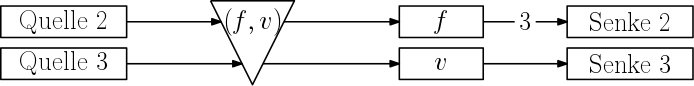
\includegraphics[width=0.8\textwidth]{faa_2_flow.png}
\end{figure}

Eine zulässige ganzzahlige Lösung $\varphi_F = (\varphi_e,\varphi_z)$ entspricht dann wieder einem FAA auf $G$. Aus der Ganzzahligkeit folgt, dass ein Winkel entweder von $\varphi_{e}$ (Ecke) oder $\varphi_{z}$ (Zuweisung) genutzt wird und somit eine Definition \ref{def_faa} respektierende Beschriftung der Winkel vorliegt.

\end{remark}


